\section{Overview}

\begin{figure}[H] 
	\centering 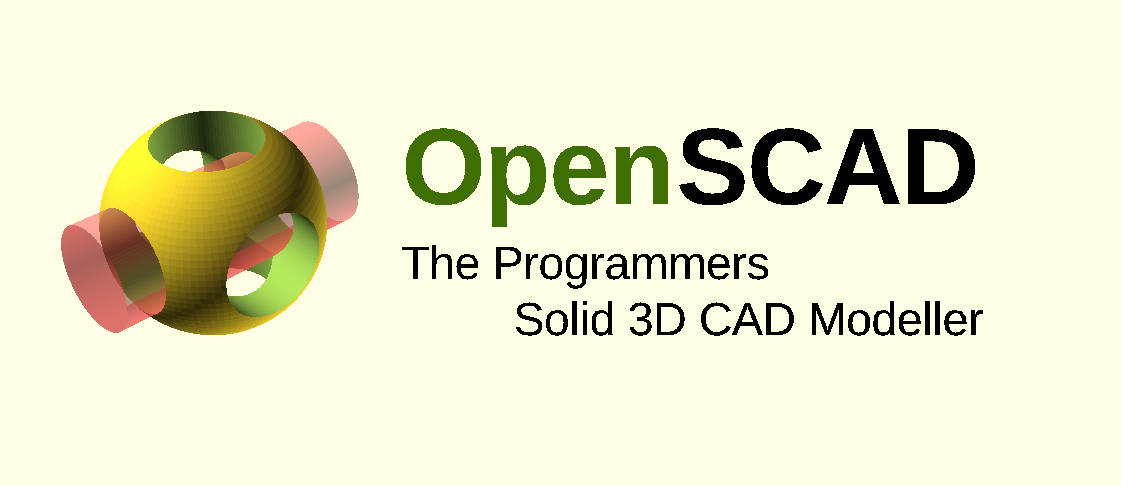
\includegraphics[scale=0.31]{images/openscad.png}
	\caption{OpenSCAD's logo}
	\label{fig:openscadlogo}
\end{figure}

User Interface for Customizing Models in OpenSCAD in which I can make my "Minor Project" in it. It is under the umbrella organization of BRL-CAD. OpenSCAD is a free and Open-source software application for creating solid 3D CAD objects. It is a script only based
modeler, with a specific description language. Parts cannot be selected or modified by mouse
in the 3D view. An OpenSCAD script specifies geometric primitives and defines how they are
modified and manipulated to render a 3D model. OpenSCAD is available for Windows, Linux and
OS X. It does constructive solid geometry (CSG). OpenSCAD has in a way redefined how easy
3D modeling can be. But the Wikipedia article on OpenSCAD says that it is a non-interactive
modeler, but rather a 3D compiler based on a textual description language. Pay attention to the
above line, its primarily what Ill be talking about. Solid 3D modeling. That sounds like some
serious business. But its just an awesome tool for making models pertaining to many uses (mostly
3D printing). And 3D printing as we can all agree upon is cool. 3D models can be created by
anyone using OpenSCAD. OpenSCAD is as much for designers as it is for you and me. What
else can most people agree upon apart from the fact that solid 3D modeling is cool? A graphical
interface is simpler and more intuitive to use. There is a general aversion for typing commands in
order to get things done. Simply put, more people have an inclination towards GUI.
